%% V1.0
%% by Gabriel Garcia, gabrcg@gmail.com
%% This is a template for Udacity projects using IEEEtran.cls

%% Be Udacious!

\documentclass[10pt,journal,compsoc]{IEEEtran}

\usepackage[pdftex]{graphicx}    
\usepackage{cite}
\usepackage{hyperref}
\usepackage{subcaption}
% \hyphenation{op-tical net-works semi-conduc-tor}

\begin{document}

\title{Map My World}

\author{Lucas Wohlhart}

\markboth{Localization project, Robotics Nanodegree Program, Udacity}%
{}
\IEEEtitleabstractindextext{%

\begin{abstract}
In this project techniques to solve the  crucial task of simultaneous localization and mapping (SLAM) will be explored. For this purpose a robot, previously designed for a localization project\cite{LWMSE6botLocalization}, is extended with regards to it's sensory capabilities. Additionally to its laser based range scanner, IMU and wheel encoders an RGB-D camera is mounted. The SLAM method used is based on RTAB-Map Real-Time Appearance-Based Mapping proposed in \cite{LabbeRTABMap}, which is graph SLAM algorithm implementing vision-based loop closure detection. To evaluate its performance, the aforementioned robot is placed in two different simulated environments, one of which is provided by Udacity and the other is created within this project. The robot is then teleoperated through the world and creates a 2D occupancy grid map and a 3D map using the SLAM algorithm.

\end{abstract}

% Note that keywords are not normally used for peerreview papers.
\begin{IEEEkeywords}
Robot, IEEEtran, Udacity, \LaTeX, Localization.
\end{IEEEkeywords}}


\maketitle
\IEEEdisplaynontitleabstractindextext
\IEEEpeerreviewmaketitle
\section{Introduction}
\label{sec:introduction}
% Introduction - Explain the concept of the project and what is trying to be achieved.
% Introduction - Student can clearly and accurately explain the problem domain.

\IEEEPARstart{T}{he} task of simultaneous localization and mapping (SLAM) is of utmost importance for the field of robotics. In the vast majority of realworld applications one cannot provide a predetermined map of the environment a robot is acting in, which is a necessity for localization and path planning. Apart from the initial nonexistence of a map, a robot also frequently operates in dynamic sceneries which means that existing maps have to be altered to accommodate changes. Therefore a map has to be generated on the fly using adequate sensors. Since the robots location is generally also unknown, SLAM can certainly be considered a chicken or egg problem.

There are various approaches to solving the SLAM problem such as Occupancy grid mapping, Fast-SLAM and GraphSLAM. The method studied in detail in this project is RTAB-Mapping (Real-Time Appearance-Based Mapping) which is a graph-based method utilizing a rangefinder sensor and an RGB-D camera.

The goal of the project is the creation of satisfactory mappings of two simulated environments by teleoperating a robot through them and estimating a 2D occupancy grid and a 3D map of the world using its sensors and the RTAB-Map algorithm.


\section{Background}

% ... as previously described, map important for localization, planning, obstacle avoidance ...
% being able 
% TODO intro with online SLAM vs full SLAM
online SLAM: estimate current pose and map based only current measurements and controls
full SLAM: estimate the poses of a trajectory and a map based all previous and current measurements and controls

% list different methods

% Background - Explain the importance of both mapping two and three dimensional space.
% Background - The student provides a sufficient background into the scope of the problem / technologically while also identifying some of the current challenges in robot mapping and why the problem domain is an important piece of robotics. They further discuss and compare mapping algorithms

\section{Scene and robot configuration}
% Scene and robot configuration - Explain how your personal Gazebo world was created and what is the layout of it. Justify your choice of robot parameters, sensor location, and how you decided to configure your package structure.
% Scene and robot configuration - Student explains how the gazebo world was created by providing an overview of the layout of items in his/her customized Gazebo world. Student also describes the robot's parameters, sensor features, and reasoning on the package structure.


\begin{figure}[thpb]
      \centering
      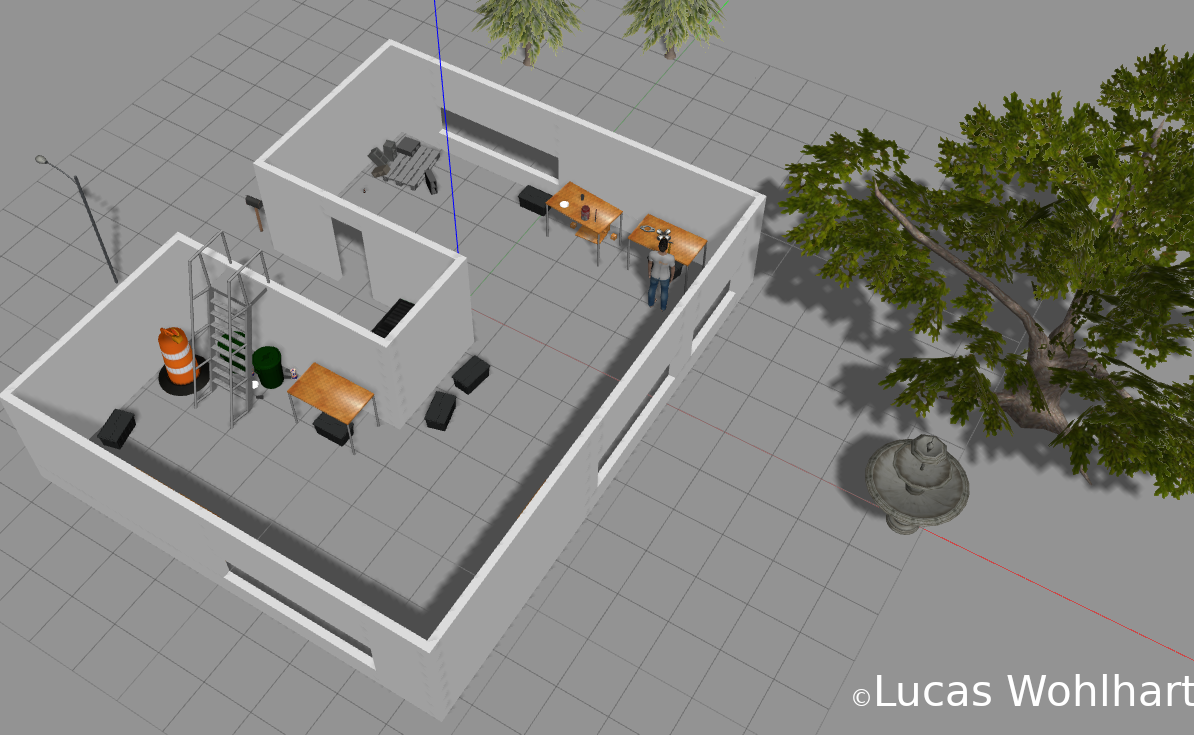
\includegraphics[width=\linewidth]{img/factory_world.png}
      \caption{Factory room world}
      \label{fig:factory_world}
\end{figure}

%\begin{figure}[thpb]
%      \centering
%      \includegraphics[width=\linewidth]{img/maze_world}
%      \caption{Maze environment}
%      \label{fig:maze}
%\end{figure}


\section{Results}

% Results - Show the results of both occupancy grid and 3D map.
% Results - The student should include the images for mapping process, final map (2D/3D) for both Gazebo worlds.

\begin{figure}
    \centering
    \begin{subfigure}[b]{0.45\textwidth}
        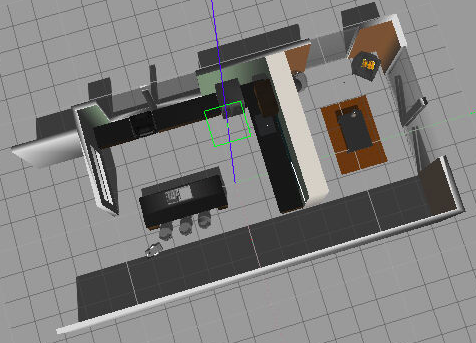
\includegraphics[width=\linewidth]{img/kitchen_map_ground_truth.png}
        \label{fig:kitchen_map_ground_truth}
    \end{subfigure}
    
    \begin{subfigure}[b]{0.45\textwidth}
        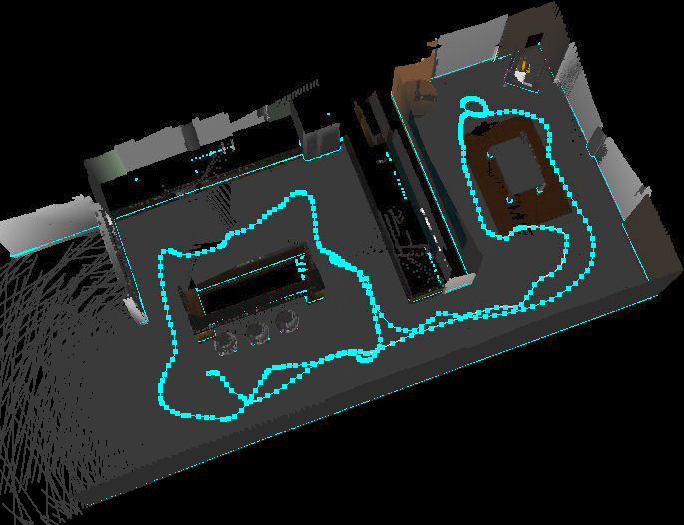
\includegraphics[width=\linewidth]{img/kitchen_map.png}
        \label{fig:kitchen_map}
    \end{subfigure}
    \caption{Kitchen dining world mapping: ground truth (top), mapping result (bottom)}    
\end{figure}

\begin{figure}[thpb]
    \centering
    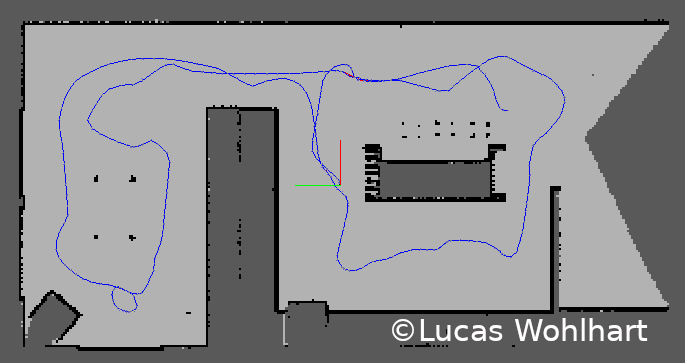
\includegraphics[width=\linewidth]{img/kitchen_occupancy_grid}
    \caption{Occupancy grid map for kitchen dining world}
    \label{fig:kitchen_occupancy_grid}
\end{figure}

\begin{figure}
    \centering
    \begin{subfigure}[b]{0.45\textwidth}
        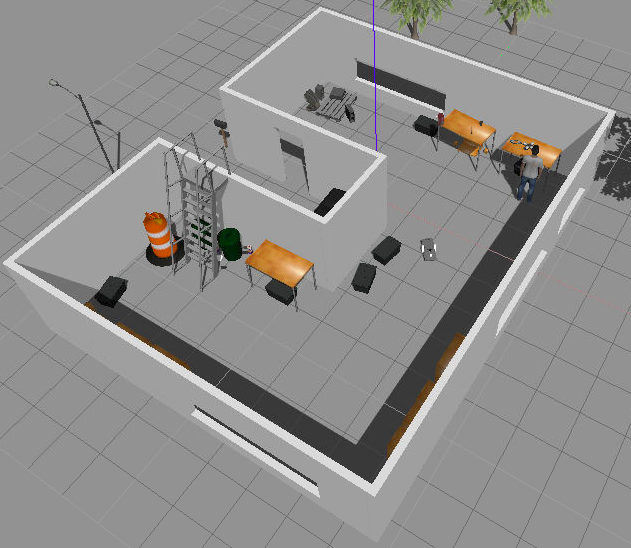
\includegraphics[width=\linewidth]{img/factory_map_ground_truth.png}
        \label{fig:factory_map_ground_truth}
    \end{subfigure}
    
    \begin{subfigure}[b]{0.45\textwidth}
        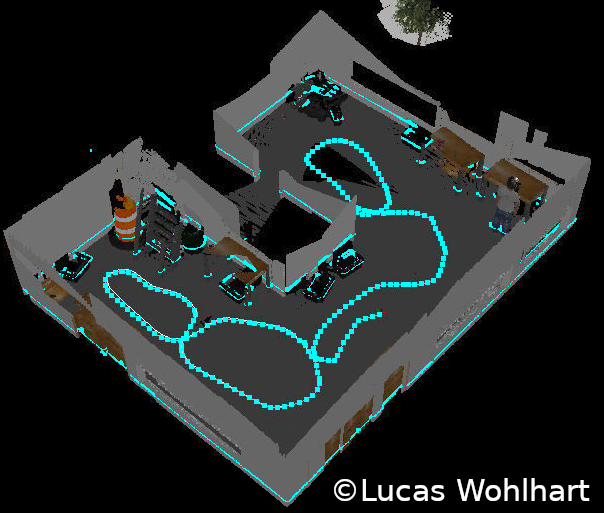
\includegraphics[width=\linewidth]{img/factory_map.png}
        \label{fig:factory_map}
    \end{subfigure}
    \caption{Factory world mapping: ground truth (top), mapping result (bottom)}    
\end{figure}

\begin{figure}[thpb]
      \centering
      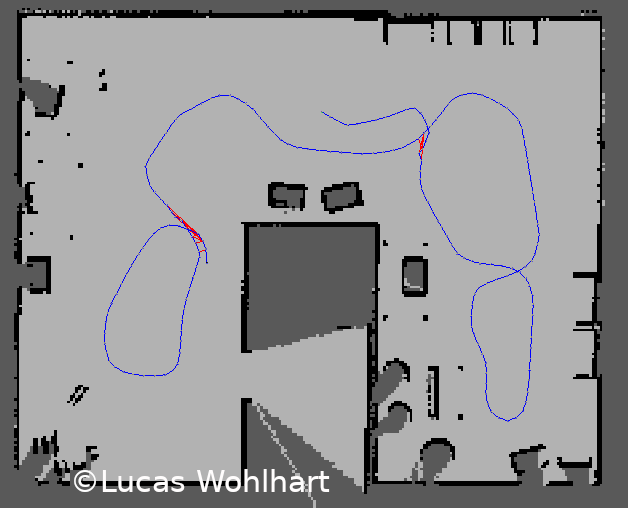
\includegraphics[width=\linewidth]{img/factory_occupancy_grid}
      \caption{Occupancy grid map for factory room world}
      \label{fig:factory_occupancy_grid}
\end{figure}

%\begin{figure}[thpb]
%      \centering
%      \includegraphics[width=\linewidth]{img/maze_world}
%      \caption{Maze environment}
%      \label{fig:maze}
%\end{figure}

\section{Discussion}
% Discussion - What went well, what went wrong. Reflect upon the results of your robot's performance, and the performance of mapping in both worlds. Justify your answers with facts.

% Discussion - The student explains how the procedure went and methodologies to improve it. The student should compare and contrast the performance of RTAB Mapping in different worlds.

\section{Conclusion / Future work}
% Future Work - Student discusses future desires with RTAB-Map. Talk about any robots and environment they applied this too.
% "Future Work - The student can discuss how they would like to leverage this tool in robotics. The student identifies other areas where mapping could be done and for what reason. Such as simulated room or physical place.
% [Optional] The student applies RTAB Mapping to a real robot."

\bibliography{bib}
\bibliographystyle{ieeetr}

\end{document}